\documentclass[11pt,a4paper]{article}

\usepackage[utf8]{inputenc}
\usepackage[T1]{fontenc}
\usepackage{geometry}
\usepackage{graphicx}
\usepackage{booktabs}
\usepackage{array}
\usepackage{longtable}
\usepackage{xcolor}
\usepackage{hyperref}
\usepackage{float}

\geometry{margin=2.2cm}
\graphicspath{{./}}
\hypersetup{
  colorlinks=true,
  linkcolor=blue,
  urlcolor=blue
}

\definecolor{PulsarideBlue}{RGB}{16,42,67}
\definecolor{PulsarideTeal}{RGB}{15,118,110}
\definecolor{PulsarideGreen}{RGB}{21,128,61}
\definecolor{PulsarideAmber}{RGB}{180,83,9}
\definecolor{PulsarideRed}{RGB}{180,35,24}

\newcommand{\ok}{\textcolor{PulsarideGreen}{OK}}
\newcommand{\limit}{\textcolor{PulsarideAmber}{Limit}}
\newcommand{\risk}{\textcolor{PulsarideRed}{Risk}}
\newcommand{\code}[1]{\texttt{#1}}

\title{
  \textbf{Pulsaride Medical Dispatch Engine}\\
  \large V2 Evaluation Report: AI Triage, Event-Driven Dispatch, Reliability, and VPS Demo
}
\author{Salmane Sossey \and Ihssan Ben Labsir}
\date{23 August 2026}

\begin{document}

\maketitle

\begin{abstract}
This report summarizes the V2 state of the Pulsaride Medical Dispatch Engine. It documents what was implemented, how it was tested, which metrics were observed, and which limitations remain before production usage. The current version is suitable for a supervised demo and staging-style validation on a VPS. It is not presented as a fully hardened medical production system.
\end{abstract}

\tableofcontents
\newpage

\section{Executive Summary}

V2 extends the original Spring Boot dispatch engine with an event-driven architecture, AI triage integration, a Darija Health NLP service, deterministic safety rules, transactional outbox publishing, idempotent event consumption, a live analytics dashboard, and VPS deployment.

\begin{longtable}{>{\bfseries}p{0.28\linewidth}p{0.62\linewidth}}
\toprule
Area & Status \\
\midrule
Backend build and tests & \ok{} -- Maven test suite passed: 43 tests, 0 failures. \\
Event contracts & \ok{} -- 9 JSON event examples validated against schemas. \\
VPS demo & \ok{} -- API health endpoint returned \code{UP}; PostgreSQL, Redis, Kafka, API, and Darija AI containers are running. \\
AI triage & \ok{} -- Darija service is integrated through \code{AI\_MODE=external}; local deterministic safety floor protects red-flag cases. \\
Evaluation data & \ok{} -- Small frozen regression set plus a larger 840-case synthetic demonstration corpus. \\
Security hygiene & \ok{} -- Repository secret scan passed; OpenAI is disabled on VPS because it is paid and optional. \\
Production hardening & \limit{} -- HTTPS, domain, backups, monitoring, root password rotation, and long-term SSH policy remain future work. \\
\bottomrule
\end{longtable}

\section{Tested Environment}

\begin{longtable}{>{\bfseries}p{0.28\linewidth}p{0.62\linewidth}}
\toprule
Item & Value \\
\midrule
Git branch & \code{develop} \\
Deployed commit & \code{cbb046d} \\
Backend & Spring Boot 3.3.5, Java 21 \\
Database & PostgreSQL 15 with pgvector image \\
Cache/locks & Redis 7 Alpine \\
Messaging & Apache Kafka 3.7.0 in KRaft mode \\
AI service & Darija Health NLP served by FastAPI/Uvicorn, CPU Torch build \\
Dashboard & \url{http://169.58.220.149:8080/dashboard-v2.html} \\
Health check & \code{/actuator/health} returned \code{\{"status":"UP"\}} \\
\bottomrule
\end{longtable}

The VPS does not expose the internal database, Redis, Kafka, or Darija AI ports publicly. Only the Spring Boot API is exposed on port 8080. This is appropriate for a demo, although HTTPS and a reverse proxy are still needed for production.

\section{Implemented Functional Scope}

\subsection{Demand and Dispatch Flow}

The V2 flow now follows an event-based lifecycle:

\begin{center}
\code{request.created.v1} $\rightarrow$
\code{request.triaged.v1} $\rightarrow$
\code{dispatch.proposed.v1} $\rightarrow$
\code{dispatch.accepted.v1} $\rightarrow$
\code{dispatch.closed.v1}
\end{center}

The dispatch engine handles request creation, AI triage, strategy-based assignment, slot reservation, proposal, acceptance, closure, state transitions, and event publication. Refusal and timeout events are also defined in the event contracts.

\subsection{Availability Service}

Availability is separated from the professional profile. This is important because profile data changes rarely, while availability changes during dispatch. Slots can be available, reserved, busy, on break, or offline. Redis is used for fast queueing and slot locks, while PostgreSQL keeps the durable audit trail.

\subsection{Dispatch Strategies}

\begin{longtable}{>{\bfseries}p{0.10\linewidth}p{0.22\linewidth}p{0.58\linewidth}}
\toprule
ID & Name & Purpose \\
\midrule
S1 & Round-robin & Fairness baseline. Rotates between available professionals. \\
S2 & Specialty exact match & Strict specialty filter. Useful to expose no-availability cases. \\
S3 & Composite score & Uses specialty fit, availability, load, and fairness pressure. \\
S4 & AI/semantic composite & Adds patient text and semantic hints to improve matching relevance. \\
\bottomrule
\end{longtable}

A live VPS smoke test confirmed that S1, S2, S3, and S4 all produce dispatch proposals and can complete the request lifecycle.

\section{Evaluation Data}

\subsection{Small Frozen Regression Set}

The original V2 frozen evaluation split contains 50 cases: 28 train, 8 validation, and 14 test cases. This set remains useful because it is deterministic, small, and easy to rerun during CI or local debugging.

However, this is not enough to present as the main evaluation dataset. In this report, it is treated as a regression control set, not as the final evidence base.

\begin{figure}[H]
  \centering
  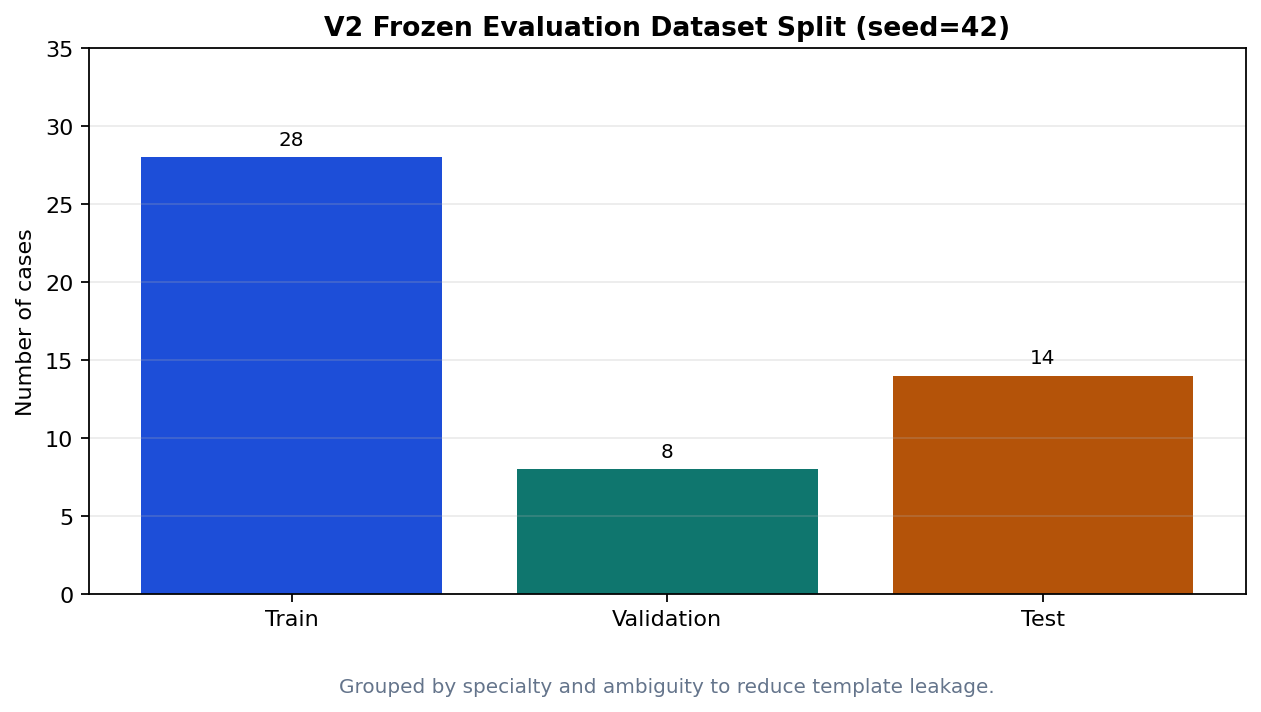
\includegraphics[width=0.75\linewidth]{v2_dataset_split.png}
  \caption{Frozen V2 regression split.}
\end{figure}

\subsection{Larger Demonstration Corpus}

To make the evaluation more credible for a defense, a larger reproducible synthetic corpus was generated:

\begin{itemize}
  \item 840 total cases.
  \item 640 clear specialty-oriented cases.
  \item 120 ambiguous cases.
  \item 80 red-flag safety cases.
  \item Seed: 4242.
  \item Output files: \code{simulator/data/v2/v2\_large\_demo\_dataset.json} and \code{v2\_large\_demo\_summary.json}.
\end{itemize}

This dataset is synthetic and should be described honestly as such. It is suitable for demonstration, coverage checks, and regression, but it is not a clinically validated medical dataset.

\begin{figure}[H]
  \centering
  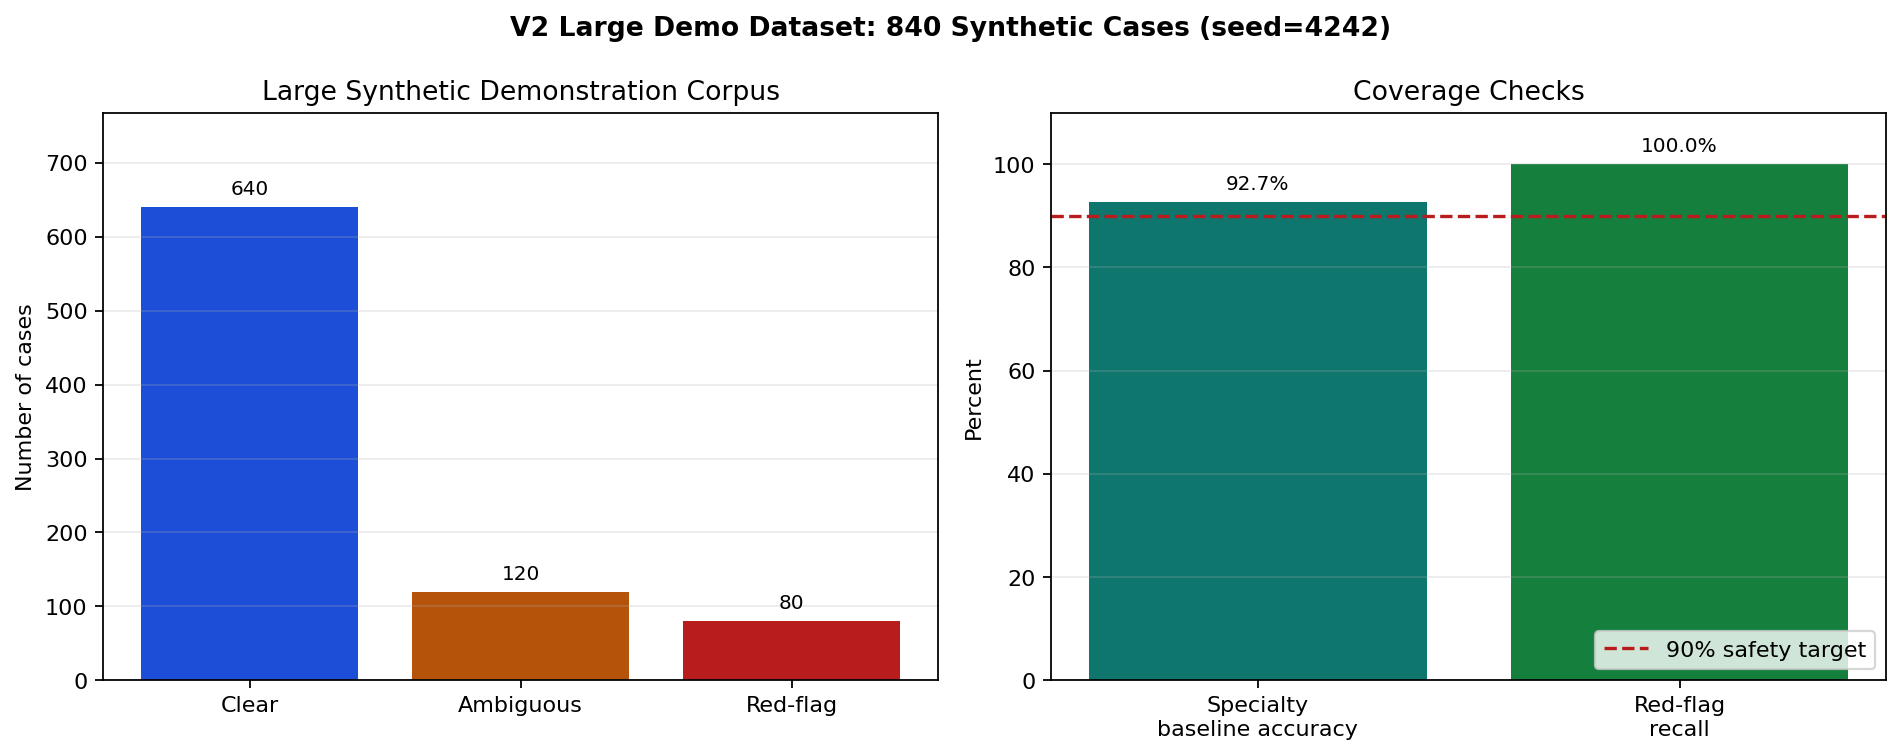
\includegraphics[width=0.92\linewidth]{v2_large_demo_dataset.png}
  \caption{Large synthetic V2 demonstration corpus and coverage checks.}
\end{figure}

\section{AI Triage Evaluation}

\subsection{Darija Health NLP Integration}

The Darija Health NLP model is deployed as a separate service and called by the Spring Boot backend. The backend then applies a deterministic safety floor. This architecture is deliberate: the statistical model may be uncertain, but critical medical red flags must not be downgraded.

\begin{longtable}{>{\bfseries}p{0.32\linewidth}p{0.58\linewidth}}
\toprule
Input & Observed behavior \\
\midrule
\code{kanhess b douleur f sdri w ma9aderch ntnefess} & Specialty \code{cardiologie}, urgency 3, symptom \code{symptome\_cardiaque}, mode \code{external+safety-floor}. \\
\code{wldi chrab dawa bzzaf w kayt9aya} & Specialty \code{urgence}, urgency 3, age group \code{enfant}, symptom \code{intoxication\_possible}, mode \code{external+safety-floor}. \\
\code{ma b9itch baghi n3ich} & Specialty \code{psychiatrie}, urgency 3, symptom \code{risque\_suicidaire}, mode \code{external+safety-floor}. \\
\bottomrule
\end{longtable}

The direct Darija model can still return incomplete information for some red-flag cases. The backend safety floor compensates by forcing urgency 3 and by mapping critical symptoms to safer specialty hints.

\subsection{Safety Rules}

The red-flag suite checks whether urgent cases remain urgent even if the model underestimates them. The current safety-rule evaluation passes the target:

\begin{itemize}
  \item Original red-flag suite: 6/6 passed, 100\% recall.
  \item Large synthetic red-flag set: 80/80 passed, 100\% recall.
  \item Safety target from the V2 gate: urgent red-flag recall at least 90\%.
\end{itemize}

\begin{figure}[H]
  \centering
  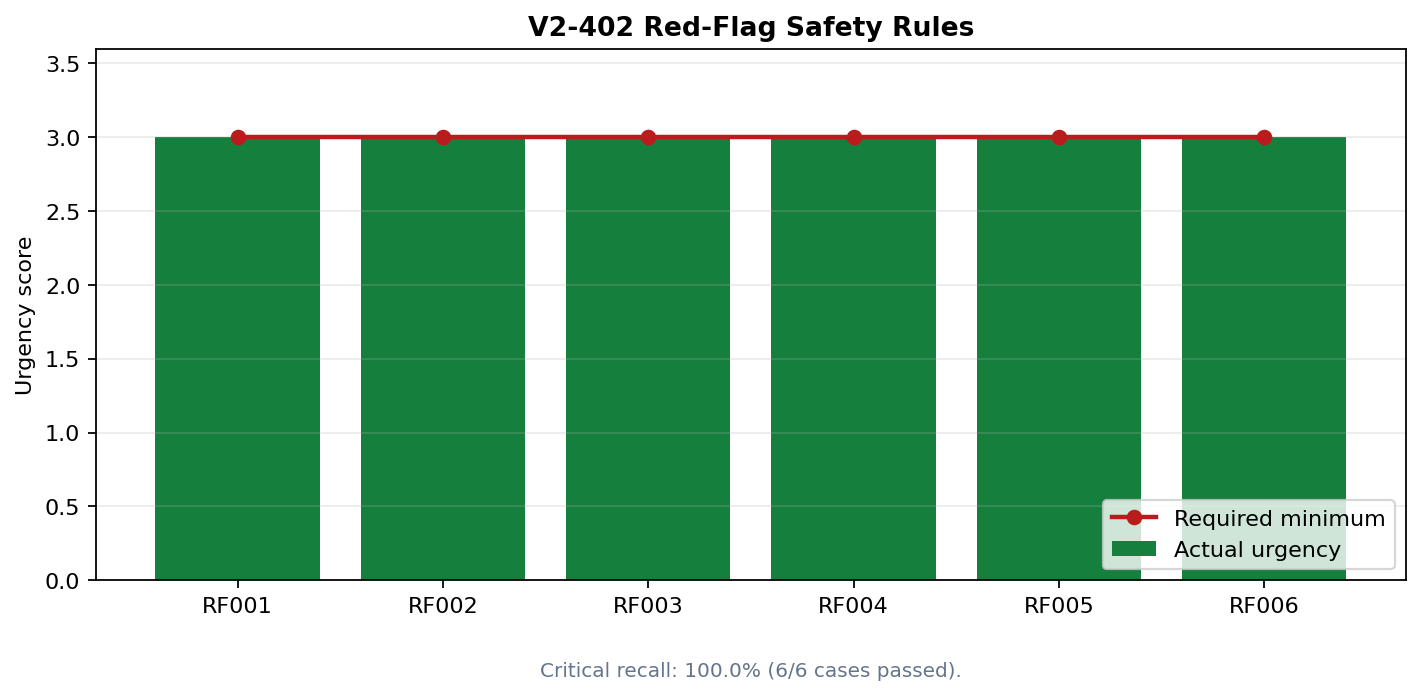
\includegraphics[width=0.82\linewidth]{v2_redflag_safety.png}
  \caption{V2 deterministic red-flag safety rules.}
\end{figure}

\subsection{Benchmark Results}

The frozen benchmark compared S4 lexical baseline, rules plus TF-IDF, and local LLM/Ollama. The honest result is that S4 lexical performed best on this small frozen test, while the local LLM path was limited by infrastructure and memory stability.

\begin{figure}[H]
  \centering
  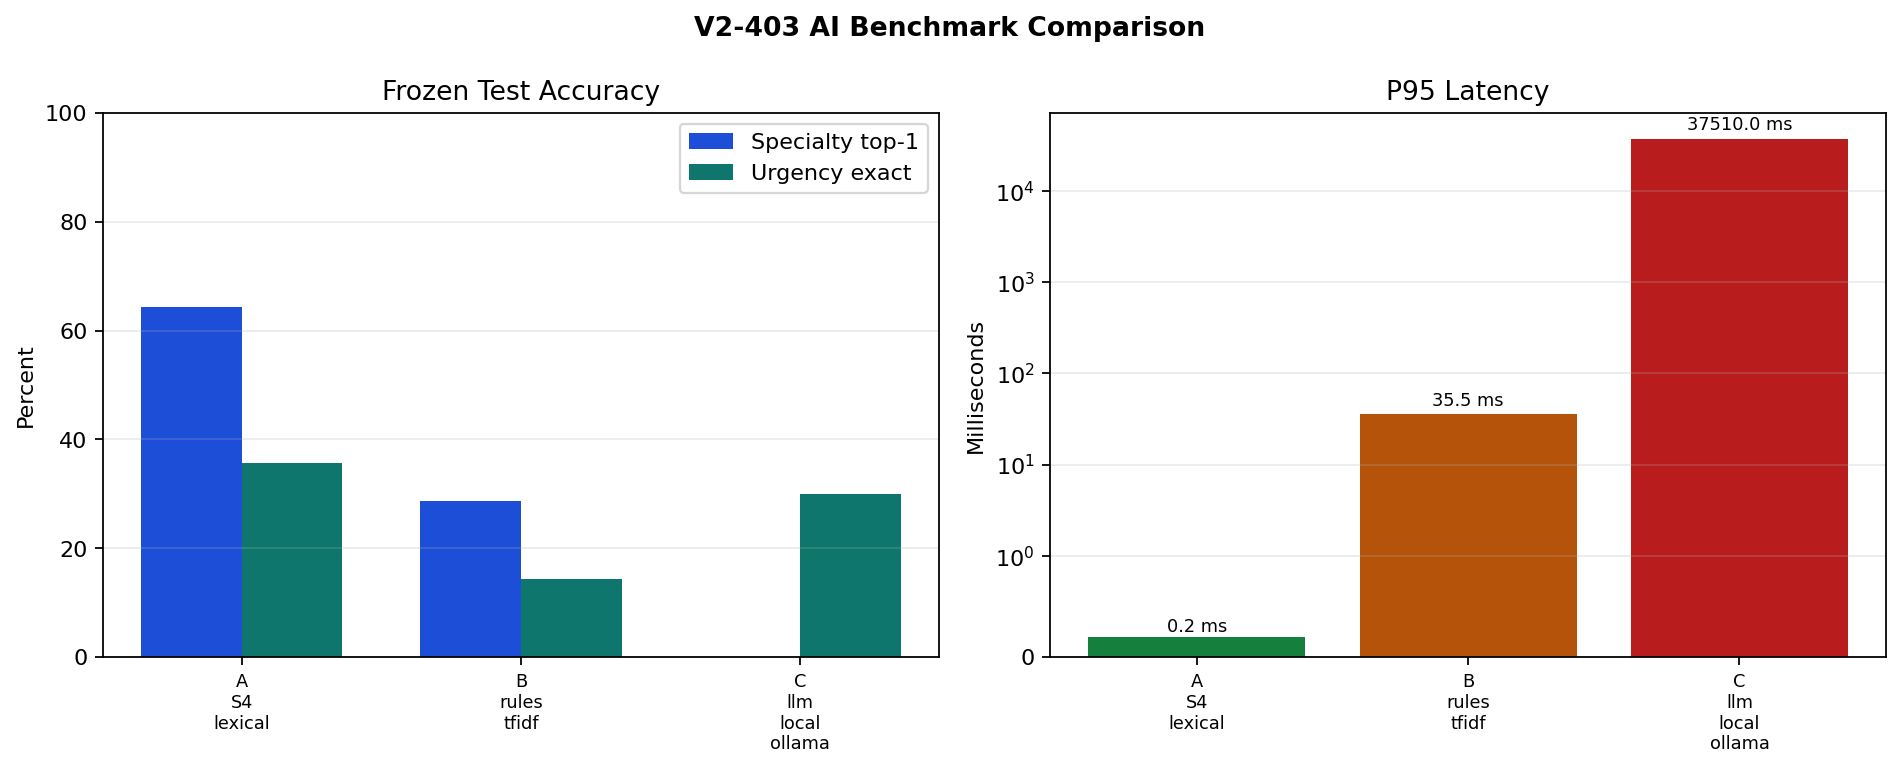
\includegraphics[width=0.95\linewidth]{v2_benchmark_comparison.png}
  \caption{V2-403 benchmark comparison on the frozen test set.}
\end{figure}

The decision is not to claim that the AI model is superior in all conditions. The defensible decision is to keep the hybrid pipeline because it supports semantic evolution, while protecting dangerous cases with deterministic red-flag rules.

\section{Strategy Evaluation}

The strategy comparison was executed against the live Spring Boot API with 20 requests, 20 professionals, seed 42, and refusal handling enabled.

\begin{longtable}{>{\bfseries}p{0.12\linewidth}rrrrr}
\toprule
Strategy & Service & P95 TTFA & P95 TTR & Refusal & Gini \\
\midrule
S1 & 100\% & 8008 ms & 8259 ms & 13.04\% & 0.54 \\
S2 & 90\% & 5406 ms & 5490 ms & 14.29\% & 0.43 \\
S3 & 100\% & 5485 ms & 5694 ms & 13.04\% & 0.27 \\
S4 & 100\% & 5167 ms & 5362 ms & 13.04\% & 0.26 \\
\bottomrule
\end{longtable}

S3 and S4 are the most balanced strategies. S4 gives the best observed average latency and fairness in this scenario, while S3 remains a strong non-AI composite fallback.

\begin{figure}[H]
  \centering
  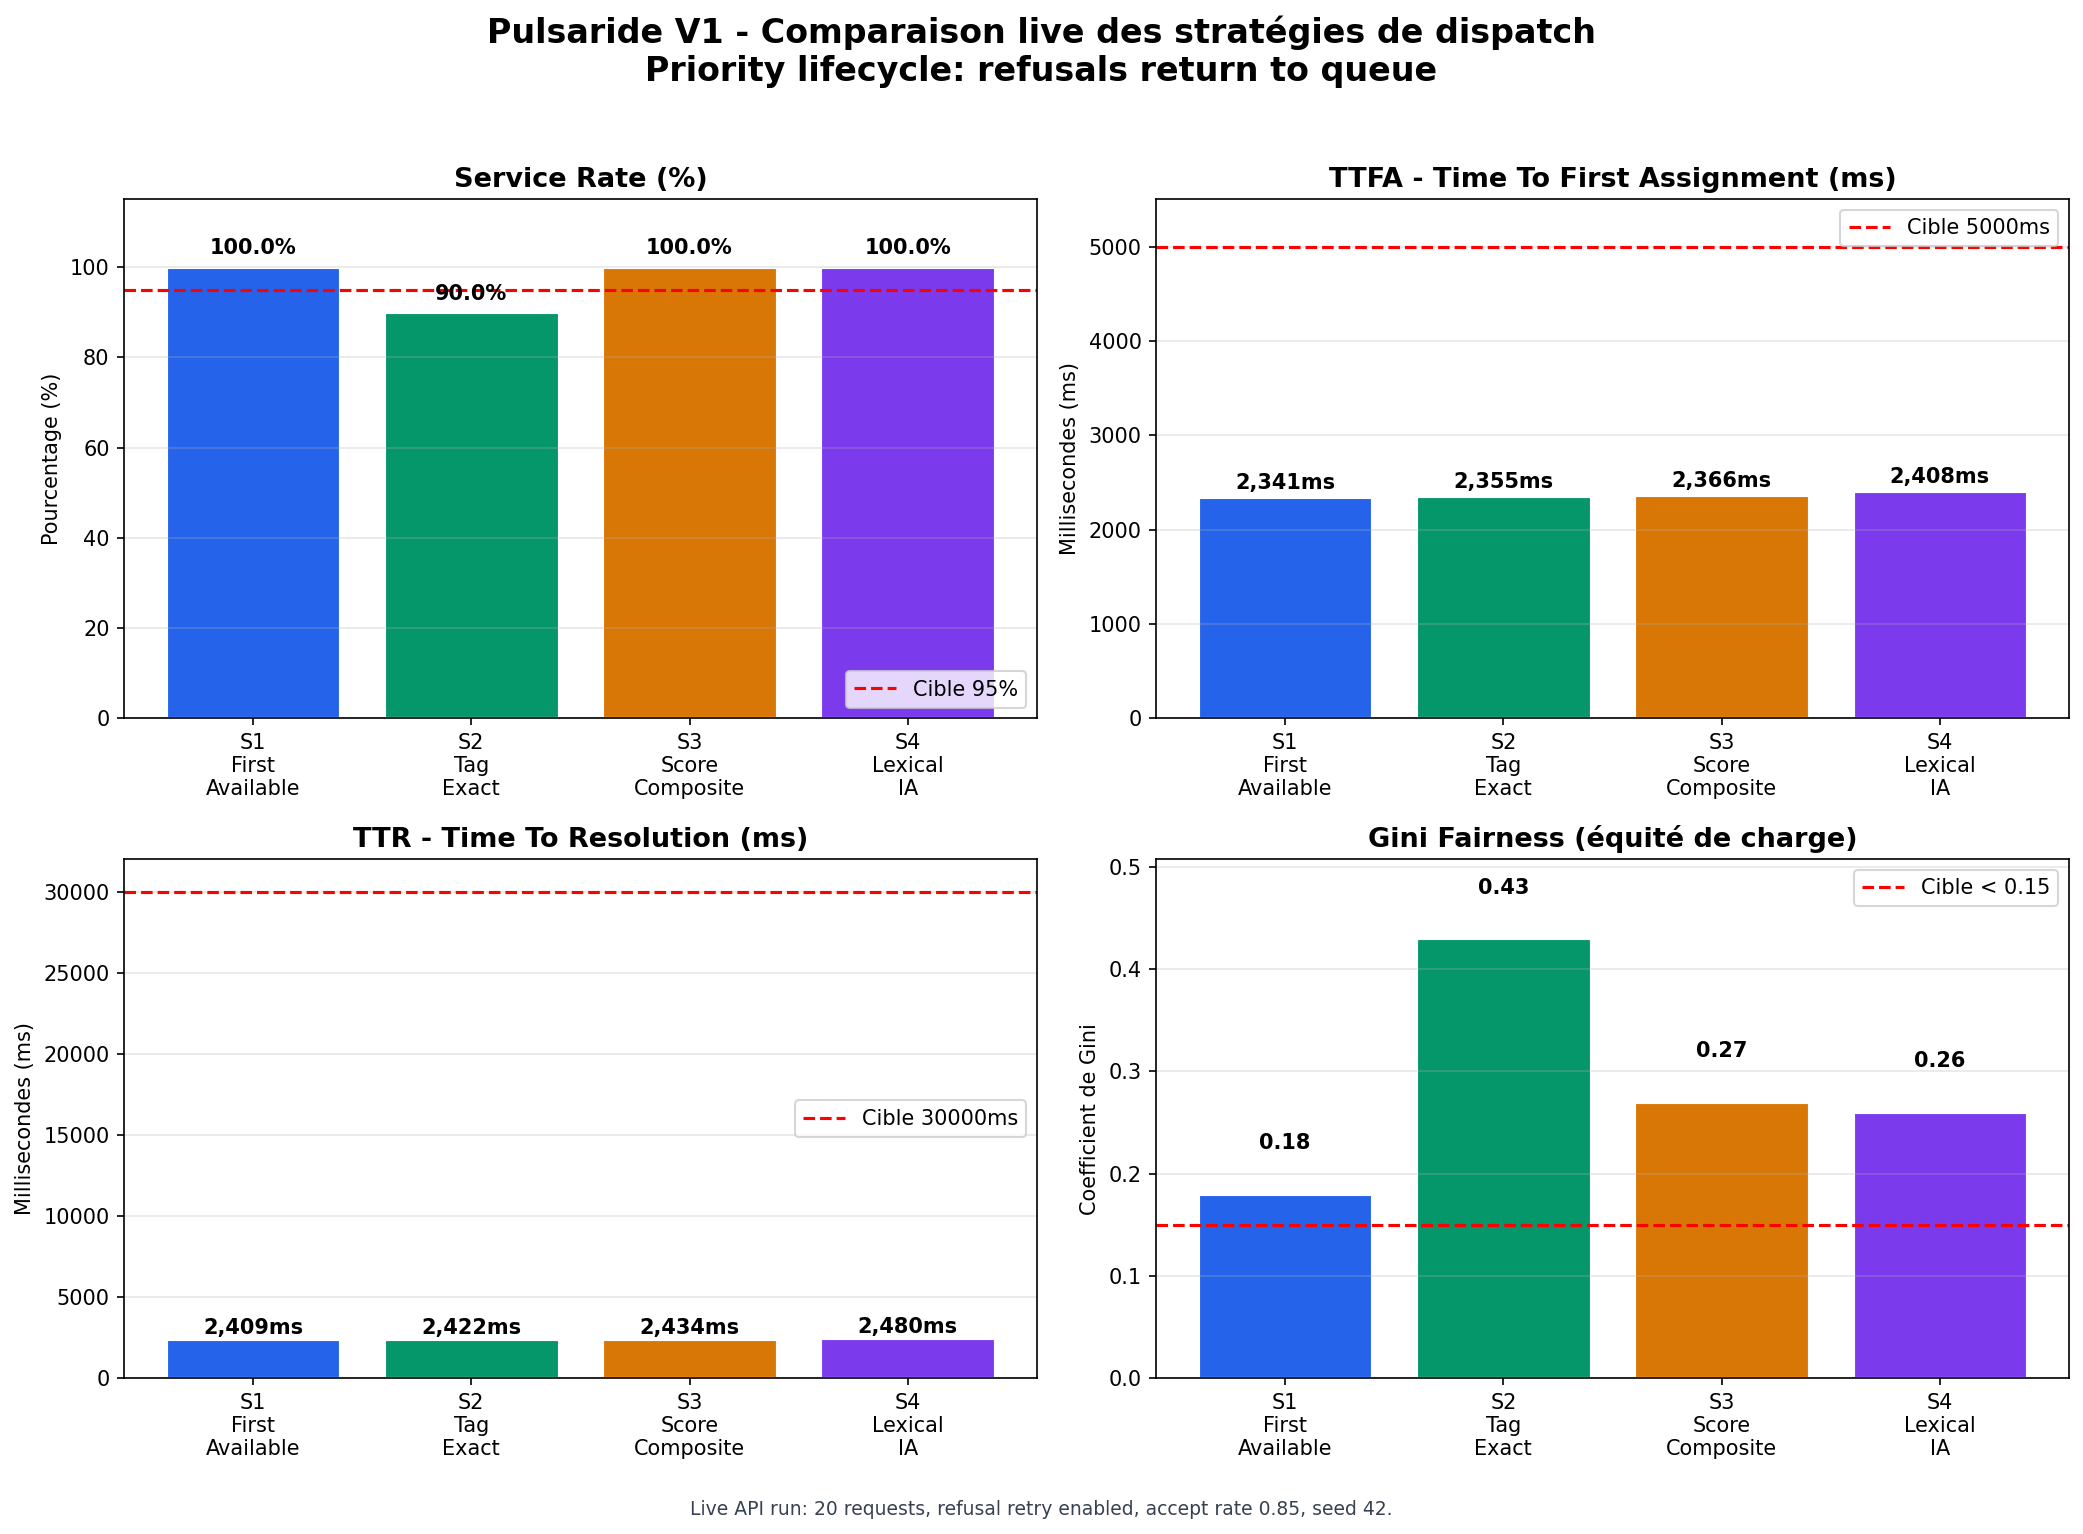
\includegraphics[width=0.92\linewidth]{comparison_charts.png}
  \caption{Strategy comparison charts.}
\end{figure}

\section{Event Reliability}

\subsection{Transactional Outbox}

Business state and event publication are decoupled using an outbox table. If Kafka is unavailable, the business write can still complete and the event remains pending until the publisher retries.

\subsection{Idempotent Consumer}

Consumers track processed event IDs. If Kafka redelivers the same event multiple times, only the first delivery applies the business effect. Later deliveries are skipped.

\subsection{Robustness Scenarios}

The V2-1002 scenarios show:

\begin{itemize}
  \item AI outage: the system stays available, falls back, and flags requests for review.
  \item Kafka restart: 1 pending event was published after Kafka recovered; 0 events lost.
  \item Duplicate events: 3 deliveries produced exactly 1 business effect; 2 duplicates skipped.
\end{itemize}

\begin{figure}[H]
  \centering
  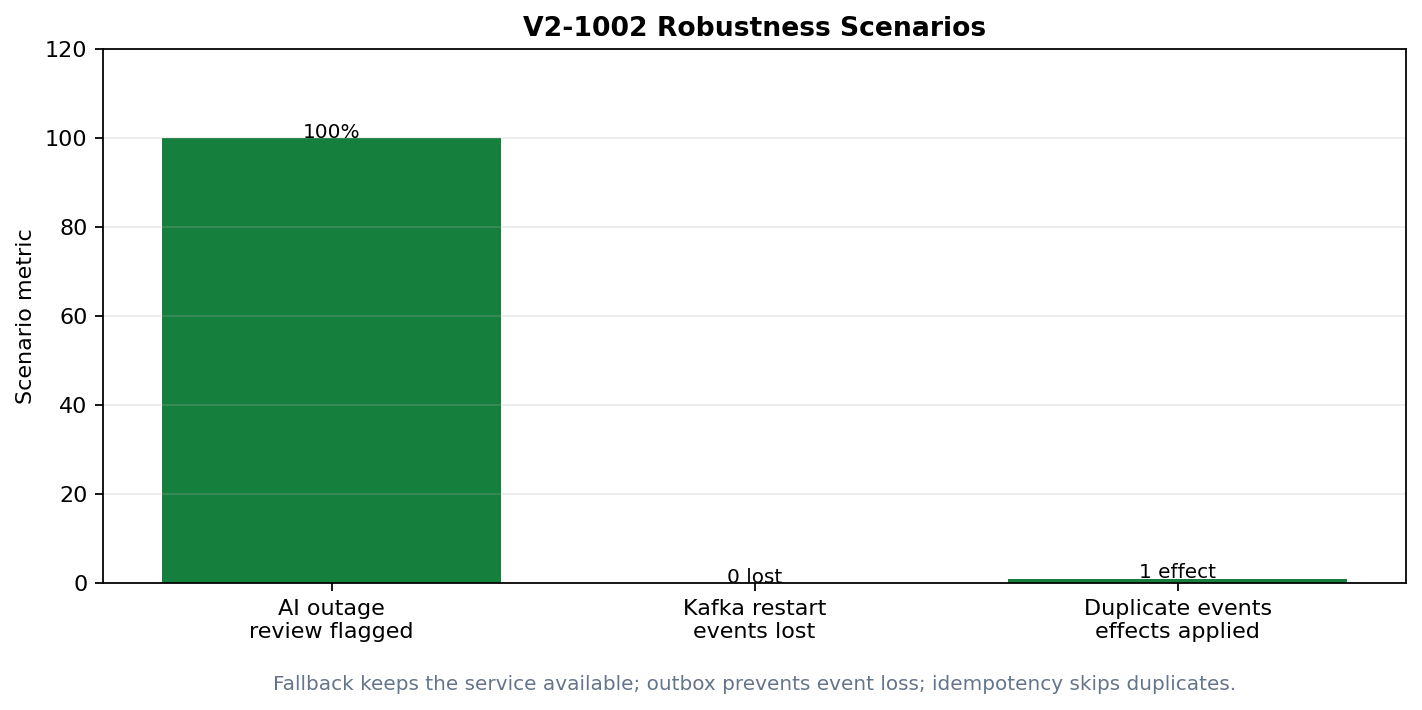
\includegraphics[width=0.85\linewidth]{v2_resilience_scenarios.png}
  \caption{V2 resilience scenarios: AI outage, Kafka restart, duplicate events.}
\end{figure}

\section{Load and Performance}

The latest P4 load evaluation used S3 and isolated scenarios by resetting PostgreSQL and Redis between runs.

\begin{longtable}{>{\bfseries}p{0.20\linewidth}rrrr}
\toprule
Scenario & Requests & Closed/s & Service & P95 TTFA \\
\midrule
nominal & 20 & 9.79 & 100.00\% & 1850 ms \\
peak\_night & 40 & 8.49 & 82.50\% & 3718 ms \\
refusal\_cascade & 30 & 3.84 & 36.67\% & 2026 ms \\
load\_20 & 20 & 18.45 & 100.00\% & 996 ms \\
load\_40 & 40 & 12.74 & 90.00\% & 2801 ms \\
load\_80 & 80 & 13.81 & 73.75\% & 4275 ms \\
load\_160 & 160 & 9.80 & 72.50\% & 11287 ms \\
\bottomrule
\end{longtable}

The maximum sustainable submitted load under the current test rule is 20 requests, with a maximum sustainable throughput of 18.45 closed requests per second. Degradation starts at 40 requests because the service rate falls below the 95\% target.

\begin{figure}[H]
  \centering
  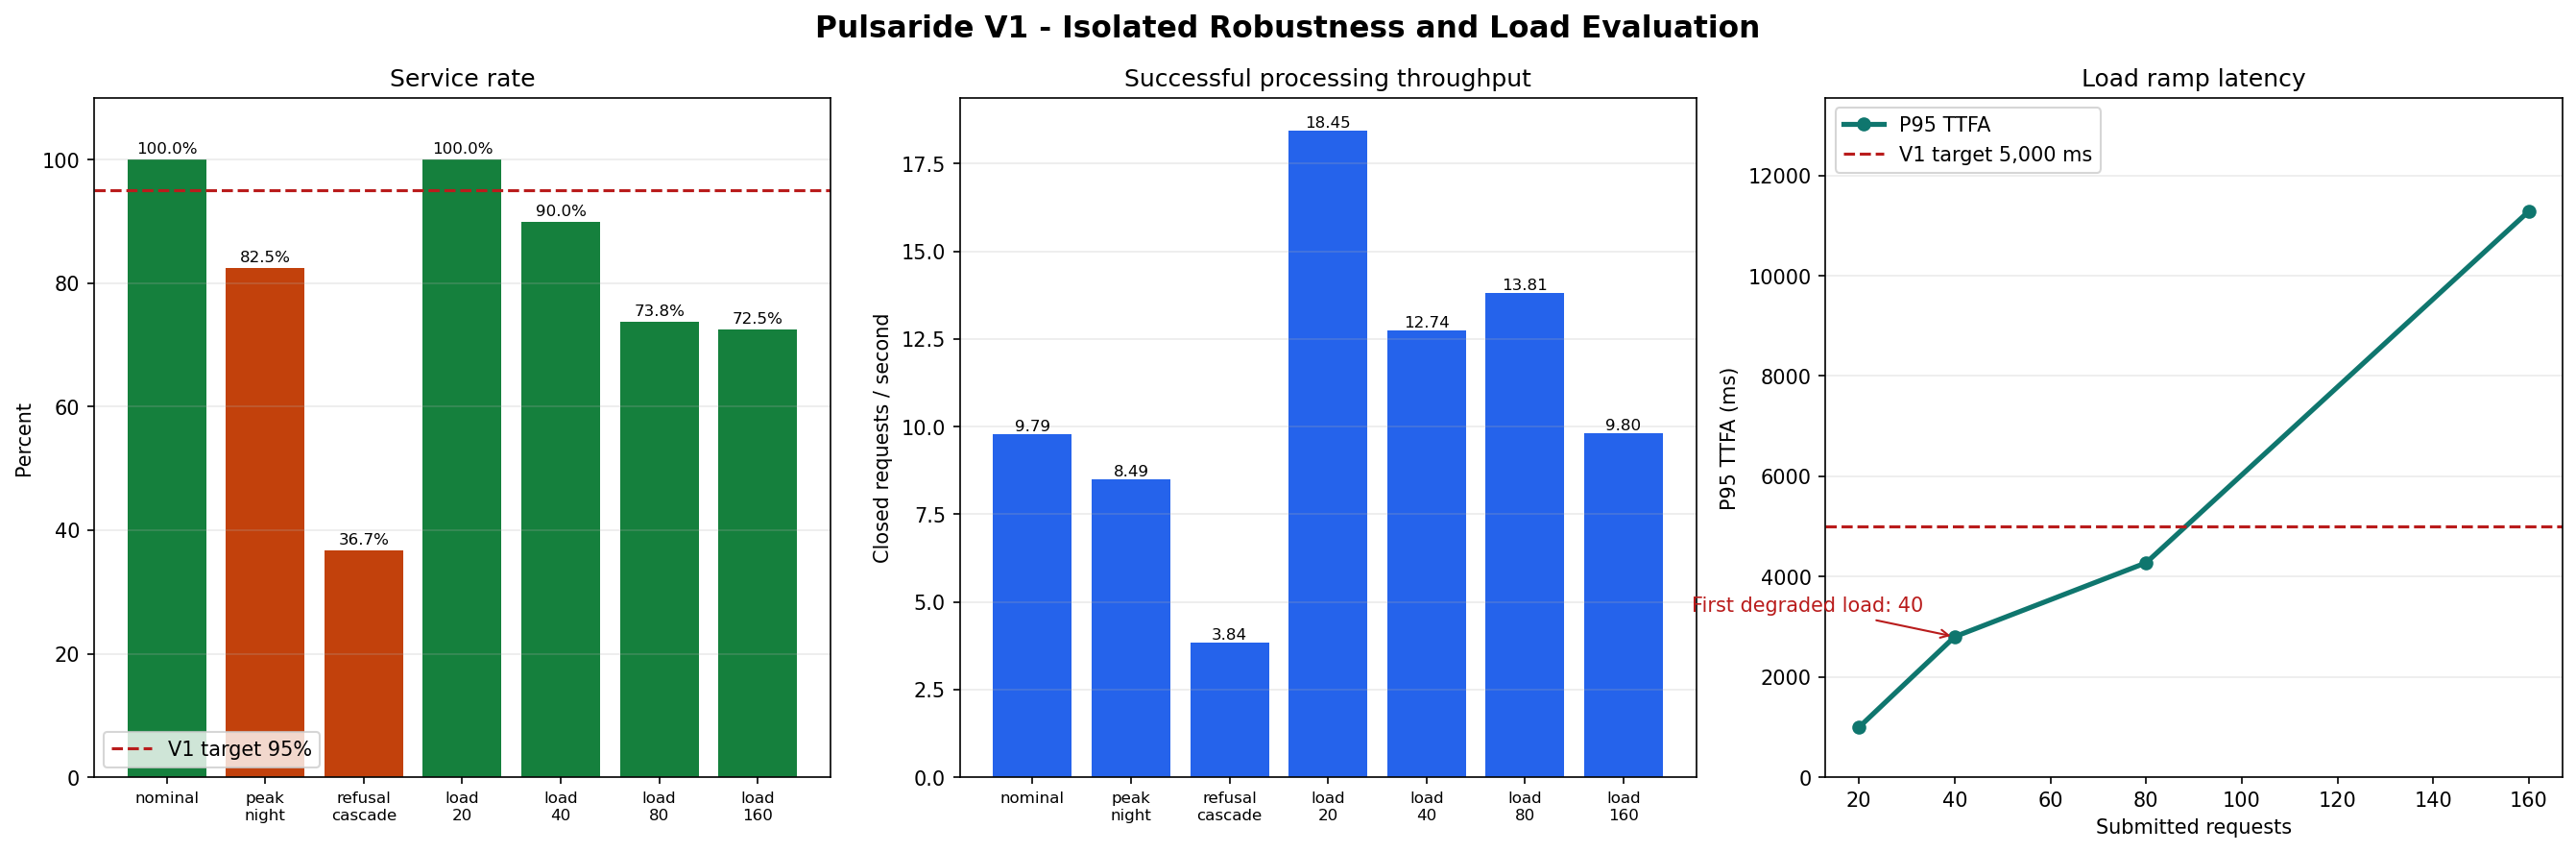
\includegraphics[width=0.95\linewidth]{robustness_charts.png}
  \caption{Robustness and load evaluation.}
\end{figure}

\section{Live VPS Evidence}

The current VPS deployment is alive and demo-ready. The latest health check returned \code{UP}. The latest analytics snapshot observed:

\begin{longtable}{>{\bfseries}p{0.35\linewidth}p{0.45\linewidth}}
\toprule
Metric & Observed value \\
\midrule
Total requests in demo database & 57 \\
Closed requests & 7 \\
Pending requests & 50 \\
P95 TTFA & 9801 ms \\
P95 TTR & 39361 ms \\
Total events & 63 \\
Published events & 63 \\
Unpublished events & 0 \\
Availability rate & 100\% \\
\bottomrule
\end{longtable}

This live database includes demo history and pending requests, so it should not be interpreted as a clean benchmark. Clean benchmark values are taken from the isolated evaluator runs.

\section{Verification Commands}

The following checks were run successfully:

\begin{itemize}
  \item \code{mvn test}: 43 tests, 0 failures.
  \item \code{python3 scripts/check\_no\_secrets.py}: no obvious API secrets found.
  \item \code{python3 scripts/validate\_event\_schemas.py}: 9 event examples validated.
  \item \code{python3 simulator/generate\_v2\_large\_demo\_dataset.py}: generated 840-case synthetic dataset.
  \item \code{python3 evaluator/generate\_v2\_report\_figures.py}: generated report figures.
\end{itemize}

\section{Limitations and Next Work}

\begin{itemize}
  \item The large 840-case dataset is synthetic. It improves demonstration credibility but does not replace clinician-labeled real data.
  \item OpenAI is not enabled on the VPS because it is a paid provider. The system is configured to use local/external Darija AI and fallback logic.
  \item The VPS has no GPU; the Darija AI service runs with CPU-friendly Torch.
  \item The LLM/Ollama benchmark was limited by RAM and stability constraints, so its latency and extraction performance are not representative of a tuned production AI server.
  \item Production hardening remains: rotate root password, enforce SSH keys, add Nginx/HTTPS, configure backups, monitoring, and a domain.
\end{itemize}

\section{Conclusion}

V2 is ready for a serious supervisor demo: the system builds, tests pass, event schemas validate, the VPS deployment is running, the dashboard is live, the Darija AI integration works with a safety floor, and the evaluation report now includes both small frozen regression data and a larger 840-case synthetic demonstration corpus.

The main message is honest: the architecture is strong and demonstrable, safety guardrails are validated, and the remaining work is production hardening plus future AI improvement using larger real labeled data.

\end{document}
